\documentclass[10pt,a4paper]{article}
\usepackage[utf8]{inputenc}
\usepackage[T1]{fontenc}
\usepackage{lmodern}
\usepackage[margin=1.8cm]{geometry}
\usepackage{graphicx,booktabs,amsmath,hyperref,caption,subcaption,enumitem,xcolor}
\hypersetup{colorlinks=true,linkcolor=black,urlcolor=blue!50!black,citecolor=black}
\captionsetup{font=small,labelfont=bf}
\setlist{nosep,leftmargin=*}
\setlength{\parskip}{3pt}\setlength{\parindent}{0pt}
\graphicspath{{../reports/figures/}}
% every number below is a macro generated by src/wikigame/report_numbers.py
% Generated by src/wikigame/report_numbers.py -- do not edit by hand.
\newcommand{\DumpDate}{20261001}
\newcommand{\NPagesTotal}{14{,}148{,}116}
\newcommand{\NLinkRows}{470{,}370{,}087}
\newcommand{\NLinktarget}{31{,}672{,}724}
\newcommand{\NNsZeroPages}{4{,}627{,}118}
\newcommand{\NRedirects}{1{,}844{,}607}
\newcommand{\NArticles}{2{,}782{,}511}
\newcommand{\NDisambig}{180{,}041}
\newcommand{\NDoubleRedirects}{97}
\newcommand{\NRedirectsDropped}{153}
\newcommand{\NLinksFromArticles}{282{,}944{,}432}
\newcommand{\ShareLinksFromArticles}{60.2\%}
\newcommand{\NRedLinks}{27{,}000{,}122}
\newcommand{\ShareRedLinks}{9.5\%}
\newcommand{\NLinksOtherNs}{17{,}180{,}988}
\newcommand{\ShareLinksOtherNs}{6.1\%}
\newcommand{\NLinksViaRedirect}{10{,}729{,}947}
\newcommand{\ShareLinksViaRedirect}{3.8\%}
\newcommand{\NCandidateEdges}{238{,}762{,}721}
\newcommand{\NSelfLoops}{53{,}339}
\newcommand{\NDuplicates}{2{,}806{,}457}
\newcommand{\ShareDuplicates}{1.18\%}
\newcommand{\NEdges}{235{,}902{,}925}
\newcommand{\NSinks}{256}
\newcommand{\NOrphans}{46{,}349}
\newcommand{\MeanOutDeg}{84.8}
\newcommand{\MedianOutDeg}{40}
\newcommand{\MedianInDeg}{14}
\newcommand{\MaxOutDeg}{5{,}374}
\newcommand{\MaxInDeg}{579{,}086}
\newcommand{\ParseSecondsPagelinks}{277}
\newcommand{\NPairs}{200{,}000}
\newcommand{\TopK}{100}
\newcommand{\Seed}{42}
\newcommand{\LsccSize}{2{,}731{,}950}
\newcommand{\LsccShare}{98.2\%}
\newcommand{\NReachable}{197{,}235}
\newcommand{\NUnreachable}{2{,}765}
\newcommand{\ShareUnreachable}{1.4\%}
\newcommand{\MeanDist}{4.09}
\newcommand{\MedianDist}{4}
\newcommand{\MaxDistSample}{29}
\newcommand{\ShareDistLeFour}{76.1\%}
\newcommand{\NCandidates}{299}
\newcommand{\NRandomBaseline}{50}
\newcommand{\OverlapOutIn}{3}
\newcommand{\OverlapOutPath}{7}
\newcommand{\OverlapInPath}{44}
\newcommand{\PathFreqKth}{307}
\newcommand{\RhoOutDetour}{0.28}
\newcommand{\RhoOutDetourP}{4.9e-06}
\newcommand{\RhoOutDetourN}{249}
\newcommand{\RhoOutOnPath}{-0.38}
\newcommand{\RhoOutOnPathP}{3.6e-10}
\newcommand{\RhoOutOnPathN}{249}
\newcommand{\RhoInDetour}{-0.58}
\newcommand{\RhoInDetourP}{8.6e-24}
\newcommand{\RhoInDetourN}{249}
\newcommand{\RhoInOnPath}{0.70}
\newcommand{\RhoInOnPathP}{2.8e-37}
\newcommand{\RhoInOnPathN}{249}
\newcommand{\RhoOutDetourAll}{-0.15}
\newcommand{\RhoOutDetourAllP}{0.0088}
\newcommand{\RhoOutDetourAllN}{299}
\newcommand{\RhoOutDetourRandom}{-0.56}
\newcommand{\RhoOutDetourRandomP}{2e-05}
\newcommand{\RhoOutDetourRandomN}{50}
\newcommand{\RhoOutDetourInGrpOut}{0.28}
\newcommand{\RhoOutDetourInGrpOutN}{100}
\newcommand{\RhoInDetourInGrpOut}{-0.84}
\newcommand{\RhoInDetourInGrpOutN}{100}
\newcommand{\RhoOutDetourInGrpIn}{-0.82}
\newcommand{\RhoOutDetourInGrpInN}{100}
\newcommand{\RhoInDetourInGrpIn}{-0.35}
\newcommand{\RhoInDetourInGrpInN}{100}
\newcommand{\RhoOutDetourInGrpPath}{-0.57}
\newcommand{\RhoOutDetourInGrpPathN}{100}
\newcommand{\RhoInDetourInGrpPath}{-0.34}
\newcommand{\RhoInDetourInGrpPathN}{100}
\newcommand{\RhoOutDetourInGrpRandom}{-0.56}
\newcommand{\RhoOutDetourInGrpRandomN}{50}
\newcommand{\RhoInDetourInGrpRandom}{-0.60}
\newcommand{\RhoInDetourInGrpRandomN}{50}
\newcommand{\RhoInDetourNoRef}{-0.86}
\newcommand{\RhoInDetourNoRefN}{192}
\newcommand{\RhoOutDetourNoRef}{0.60}
\newcommand{\RhoOutDetourNoRefN}{192}
\newcommand{\NReferenceCandidates}{57}
\newcommand{\MinTypeSize}{5}
\newcommand{\NSmallTypes}{6}
\newcommand{\NSmallTypePages}{12}
\newcommand{\SmallTypesList}{continent, discipline, organisation, other, person, territory}
\newcommand{\NTypeLabels}{14}
\newcommand{\TopOverlapK}{50}
\newcommand{\TopOverlapOutDetour}{2}
\newcommand{\TopOverlapOutOnPath}{2}
\newcommand{\GrpOutMedDetour}{3.02}
\newcommand{\GrpOutOnPath}{0.8\%}
\newcommand{\GrpInMedDetour}{1.99}
\newcommand{\GrpInOnPath}{3.0\%}
\newcommand{\GrpPathMedDetour}{1.52}
\newcommand{\GrpPathOnPath}{4.2\%}
\newcommand{\GrpRandomMedDetour}{3.91}
\newcommand{\GrpRandomOnPath}{0.0\%}
\newcommand{\NotRankable}{0}
\newcommand{\MinCoverage}{90\%}
\newcommand{\NUnreachTOrphan}{2{,}494}
\newcommand{\NUnreachTOutside}{2{,}759}
\newcommand{\NUnreachSOutside}{47}
\newcommand{\NUnreachSSink}{6}
\newcommand{\NDistGeEight}{78}
\newcommand{\NDistinctOnPaths}{155{,}967}
\newcommand{\PathFreqTies}{1}
\newcommand{\GrpOutMedOnPath}{0.08\%}
\newcommand{\GrpInMedOnPath}{1.94\%}
\newcommand{\GrpPathMedOnPath}{3.49\%}
\newcommand{\GrpRandomMedOnPath}{0.00\%}
\newcommand{\NSexagenary}{14}
\newcommand{\SexagenaryMedOutDeg}{2{,}523}
\newcommand{\SexagenaryMedDetour}{3.37}
\newcommand{\SexagenaryMedInDeg}{44.5}
\newcommand{\TopFifteenTypes}{10 country, 3 city, 1 continent, 1 period}
\newcommand{\NBfsRuns}{200{,}598}
\newcommand{\RawGB}{2.76}
\newcommand{\BestHub}{France}
\newcommand{\BestHubDetour}{0.92}
\newcommand{\BestHubOnPath}{24.5\%}
\newcommand{\TopOutHub}{Liste des cantons français au Grand Est depuis 2015}
\newcommand{\TopOutHubDetour}{4.20}
\newcommand{\TopOutHubRank}{285}
\newcommand{\TypeCityN}{15}
\newcommand{\TypeCityMedDetour}{1.64}
\newcommand{\TypeConceptN}{12}
\newcommand{\TypeConceptMedDetour}{2.39}
\newcommand{\TypeContinentN}{2}
\newcommand{\TypeContinentMedDetour}{1.40}
\newcommand{\TypeCountryN}{42}
\newcommand{\TypeCountryMedDetour}{1.42}
\newcommand{\TypeDisciplineN}{3}
\newcommand{\TypeDisciplineMedDetour}{1.69}
\newcommand{\TypeLanguageN}{6}
\newcommand{\TypeLanguageMedDetour}{2.93}
\newcommand{\TypeListN}{67}
\newcommand{\TypeListMedDetour}{2.97}
\newcommand{\TypeOrganisationN}{1}
\newcommand{\TypeOrganisationMedDetour}{2.87}
\newcommand{\TypeOtherN}{2}
\newcommand{\TypeOtherMedDetour}{2.65}
\newcommand{\TypePeriodN}{38}
\newcommand{\TypePeriodMedDetour}{1.65}
\newcommand{\TypePersonN}{1}
\newcommand{\TypePersonMedDetour}{2.21}
\newcommand{\TypeReferenceN}{57}
\newcommand{\TypeReferenceMedDetour}{2.50}
\newcommand{\TypeTerritoryN}{3}
\newcommand{\TypeTerritoryMedDetour}{1.79}
\newcommand{\RedirTopMedShare}{0.06\%}
\newcommand{\RedirTopMaxShare}{2.7\%}
\newcommand{\RedirTopMaxTitle}{Première Guerre mondiale}
\newcommand{\RedirRhoInDirect}{0.988}
\newcommand{\RedirTopTwentyInOverlap}{20}
\newcommand{\RedirRhoInDetourDirect}{-0.58}
\newcommand{\BiasTopN}{100}
\newcommand{\BiasTopMedShare}{0.5\%}
\newcommand{\BiasTopMeanShare}{8.9\%}
\newcommand{\BiasTopMedAll}{2{,}524}
\newcommand{\BiasTopMedBody}{2{,}520.5}
\newcommand{\BiasTopMedDump}{2{,}524}
\newcommand{\BiasInN}{50}
\newcommand{\BiasInMedShare}{23.9\%}
\newcommand{\BiasInMeanShare}{29.5\%}
\newcommand{\BiasInMedAll}{352}
\newcommand{\BiasInMedBody}{223.5}
\newcommand{\BiasInMedDump}{352}
\newcommand{\BiasRandomN}{50}
\newcommand{\BiasRandomMedShare}{26.1\%}
\newcommand{\BiasRandomMeanShare}{35.6\%}
\newcommand{\BiasRandomMedAll}{55.5}
\newcommand{\BiasRandomMedBody}{30}
\newcommand{\BiasRandomMedDump}{55.5}
\newcommand{\BiasRho}{0.90}
\newcommand{\BiasErrors}{0}
\newcommand{\BiasNPages}{200}
\newcommand{\BiasRatioMed}{1.000}
\newcommand{\BiasRatioMin}{0.993}
\newcommand{\BiasRatioMax}{1.014}
\newcommand{\CsrLoadS}{5.5}
\newcommand{\CsrBfsS}{3.4}
\newcommand{\CsrRevBfsS}{3.3}
\newcommand{\CsrDiskGB}{2.03}
\newcommand{\CsrRamGB}{2.7}
\newcommand{\DuckLoadS}{0.02}
\newcommand{\DuckBfsS}{9.4}
\newcommand{\DuckRevBfsS}{12.0}
\newcommand{\DuckDiskGB}{1.53}
\newcommand{\DuckRamGB}{2.4}
\newcommand{\DuckBfsRatio}{2.8}
\newcommand{\DuckRevBfsRatio}{3.6}
\newcommand{\OtherSeed}{69}
\newcommand{\SeedN}{245}
\newcommand{\SeedRho}{0.99998}
\newcommand{\SeedRhoOnPath}{0.9990}
\newcommand{\SeedMaxDiff}{0.005}
\newcommand{\SeedTopFifteenShared}{15}
\newcommand{\SeedTopFifteenOrder}{in the same order}
\newcommand{\OtherBestHub}{France}
\newcommand{\OtherBestHubDetour}{0.92}
\newcommand{\OtherBestHubOnPath}{24.3\%}
\newcommand{\OtherNCandidates}{299}
\newcommand{\OtherMeanDist}{4.09}
\newcommand{\OtherShareUnreachable}{1.4\%}
\newcommand{\OtherRhoOutDetour}{0.29}
\newcommand{\OtherRhoInDetour}{-0.58}
\newcommand{\SeedSharedCandidates}{245}
\newcommand{\RobustN}{272}
\newcommand{\RobustRho}{0.9998}
\newcommand{\RobustMaxDiff}{0.045}
\newcommand{\PairsOldN}{2{,}000}
\newcommand{\PairsOldSeconds}{946}
\newcommand{\PairsNewN}{198{,}000}
\newcommand{\PairsNewSeconds}{329}
\newcommand{\PairRateOld}{2.1}
\newcommand{\PairRateNew}{601}
\newcommand{\PairSpeedup}{284}
\newcommand{\NEligible}{2{,}602{,}470}
\newcommand{\AllPairsTrillions}{6.8}
\newcommand{\AllPairsYearsBidir}{357}
\newcommand{\FullBfsWallS}{1.0}
\newcommand{\AllPairsDaysBfs}{30}
\newcommand{\AllPairsTB}{6.8}

\newcommand{\obs}{\textbf{Observation.}~}
\newcommand{\interp}{\textbf{Interpretation.}~}

\title{\vspace{-1.2cm}Landmarks of the Wikipedia game:\\ are the pages players aim for the best hubs?}
\author{Raphaël Hazan, Nicolas Salapete, Edouard Souied, Josh Soussan\\
\small Data, Data Storage, Data Collection --- CentraleSupélec / Université Paris-Saclay}
\date{\small Dump of French Wikipedia dated \DumpDate{} --- code and data instructions in the repository (\texttt{README.md})}

\begin{document}
\maketitle
\vspace{-0.6cm}

\section{Question and approach}
In the Wikipedia game, a player must go from a start article to a target article by clicking
internal links only. Players typically head for \emph{landmarks}: countries, general pages, pages
with many links. They then "descend" towards the target. \textbf{Are these intuitive
landmarks actually the best hubs for connecting any two articles, and if not, which pages are?}

We build the complete directed link graph of French Wikipedia and compare two criteria.
\begin{itemize}
\item The \emph{perceived} criterion: a page's out-degree (number of distinct articles it links to),
  plus a type label (country, city, list, \dots).
\item The \emph{real} criterion, computed on random pairs $(s,t)$ with $d(s,t)<\infty$:
  \begin{itemize}
  \item the \textbf{mean detour} $d(s,h)+d(h,t)-d(s,t)$, i.e. the extra clicks a player pays for
    going through $h$;
  \item the \textbf{on-shortest-path rate}, the share of pairs with a detour of 0. This counts
    the pairs for which $h$ lies on \emph{at least one} shortest path, so ties need no arbitrary
    rule.
  \end{itemize}
\end{itemize}
Only BFS, descriptive statistics and rank comparisons are used.

\section{Data and provenance}
We acquired the official Wikimedia database dumps of \texttt{frwiki} dated \DumpDate. This was the
most recent complete dump, checked in \texttt{dumpstatus.json}.
\begin{itemize}
\item \textbf{Tables.} \texttt{page}, \texttt{pagelinks}, \texttt{linktarget}, \texttt{redirect} and
  \texttt{page\_props}: \RawGB\,GB compressed, CC BY-SA, no personal data.
\item \textbf{Download.} \texttt{download.py} streams the files with resume support and verifies
  each one against the official SHA-1 file.
\item \textbf{Parsing.} A custom streaming parser (\texttt{parse\_sql.py}) reads each file's
  \texttt{CREATE TABLE} statement instead of assuming the schema. This mattered: the
  2026 dumps changed layout, with one row per line. Any unexpected syntax raises an error instead
  of shifting columns.
\item \textbf{Validation.} The parser keeps all \NLinkRows{} \texttt{pagelinks} rows (parsed in
  \ParseSecondsPagelinks\,s). An independent \texttt{zcat|grep} count gives exactly the same totals
  for all five tables, and the parser has unit tests on tricky rows.
\item \textbf{Secondary collection.} For a bias check, we fetched the rendered HTML of
  \BiasNPages{} pages through the MediaWiki API. We asked for the exact revision of the dump
  (\texttt{oldid}), at a polite rate, with responses cached.
\end{itemize}
Known limitations: the graph is a snapshot; it includes links generated by templates; the link
tables are updated asynchronously.

\section{Cleaning: measured problems and decisions}
We measured first (\texttt{quality.json}) and then transformed. Table~\ref{tab:clean}
pairs each measured problem with its effect on our use and the decision taken. The resulting graph
has \textbf{\NArticles{} nodes and \NEdges{} edges}.
\begin{itemize}
\item Degrees: mean out-degree \MeanOutDeg, median out-degree \MedianOutDeg, median in-degree
  \MedianInDeg.
\item Disambiguation pages (\NDisambig) stay traversable but are never drawn as start or target.
\item Sinks (\NSinks) and orphans (\NOrphans) are kept and reported.
\end{itemize}

\begin{table}[h]\centering\small
\begin{tabular}{@{}p{6.4cm}p{4.6cm}p{5.6cm}@{}}\toprule
Measured problem & Effect on shortest paths & Decision \\\midrule
\NPagesTotal{} pages, only \NNsZeroPages{} in the main namespace, of which \NRedirects{} redirects & non-article pages cannot be visited in the game & nodes = namespace-0 non-redirects (\NArticles) \\
\NLinksViaRedirect{} links from articles (\ShareLinksViaRedirect) point to a redirect; \NDoubleRedirects{} double redirects, no cycles & dropping them removes real paths; keeping redirect nodes adds a fake click & resolve chains (max depth 5, measured max 3); \NRedirectsDropped{} broken / out-of-namespace redirects dropped \\
\NRedLinks{} red links (\ShareRedLinks) and \NLinksOtherNs{} links to other namespaces (\ShareLinksOtherNs) & impossible moves & dropped \\
\NSelfLoops{} self-loops and \NDuplicates{} duplicates (\ShareDuplicates) after redirect resolution & no effect on distances; distort degrees & dropped (simple directed graph) \\
\bottomrule\end{tabular}
\caption{Quality problems measured on the dump (from \texttt{quality.json}) and the transformation each one justifies.}
\label{tab:clean}
\end{table}
\vspace{-0.4cm}

\section{Storage choice}
Our workload is full BFS runs over a static graph (two per candidate hub, plus the pair
distances), and degree and title lookups.
We benchmarked two options on these exact queries (Table~\ref{tab:storage}):
\begin{itemize}
\item NumPy CSR adjacency arrays with a Parquet node table;
\item a DuckDB database with edge tables sorted by source and by target, where the BFS is a SQL
  query per level and its result is checked against the NumPy BFS.
\end{itemize}

\begin{table}[h]\centering\small
\begin{tabular}{@{}lrr@{}}
\toprule
Measure & NumPy CSR + Parquet & DuckDB \\
\midrule
Build from cleaned edges (s) & 44 & 29 \\
Disk size (GB) & 2.03 & 1.53 \\
Load / connect (s) & 5.5 & 0.02 \\
Peak resident memory (GB) & 2.7 & 2.4 \\
Q1 full forward BFS (s) & 3.4 & 9.4 \\
Q2 full reverse BFS (s) & 3.3 & 12.0 \\
Q3 degrees of 1000 nodes (ms) & 0.06 & 12.4 \\
Q4 2000 title/id lookups (ms) & 0.4 & 1515 \\
\bottomrule
\end{tabular}

\caption{Storage benchmark on our queries (fresh process per option, same cleaned edge list).}
\label{tab:storage}
\end{table}
\vspace{-0.3cm}

\obs DuckDB is smaller on disk and opens instantly. CSR is \DuckBfsRatio$\times$ faster on
forward BFS, \DuckRevBfsRatio$\times$ faster on reverse BFS, and orders of magnitude faster on
lookups. Peak memory is similar.

\textbf{Choice.} We keep CSR. Its contiguous neighbour lists match the BFS access pattern, \CsrDiskGB\,GB
fit in RAM, and the open \texttt{.npy}/Parquet formats need no server. DuckDB remains the right
tool for the relational part: the out-of-core cleaning joins over 470\,M rows. Neo4j was discussed
but not benchmarked. It requires a server, and its transactional design brings nothing for full
BFS on a read-only graph.

\section{Analysis method}
\begin{itemize}
\item \textbf{Pairs.} We draw \NPairs{} pairs $(s,t)$ uniformly among non-disambiguation articles
  (seed \Seed). Each pair distance is exact, computed by a bidirectional BFS (validated against the plain BFS). A persistent cache lets new
  samples reuse every computation and never redraw old pairs.
\item \textbf{Candidates.} The candidate hubs are the union of four sets, \NCandidates{} pages in
  total:
  \begin{itemize}
  \item the top-\TopK{} pages by out-degree (\emph{perceived});
  \item the top-\TopK{} by in-degree;
  \item the top-\TopK{} by frequency on one sampled shortest path per pair (random tie-break, used
    only to \emph{discover} candidates);
  \item \NRandomBaseline{} random articles as a baseline. Restricting the comparison to high-degree
    pages would hide the range of hub quality.
  \end{itemize}
\item \textbf{Hub metrics.} Each candidate gets a forward and a reverse BFS, which give $d(h,\cdot)$
  and $d(\cdot,h)$ for all nodes and hence its detour on every pair. All candidates are connected
  to at least \MinCoverage{} of the pairs, so all of them are ranked (\NotRankable{} excluded).
\end{itemize}

\section{Results}
\subsection{Observations}
\begin{itemize}
\item \textbf{The graph is tightly connected.}
  \begin{itemize}
  \item The largest strongly connected component holds \LsccSize{} articles (\LsccShare).
  \item Of the random pairs, \NUnreachable{} (\ShareUnreachable) have no path. The target lies
    outside that component in \NUnreachTOutside{} of them (an orphan in \NUnreachTOrphan), and
    the start lies outside it in \NUnreachSOutside.
  \item Reachable pairs are \MeanDist{} clicks apart on average (median \MedianDist), and
    \ShareDistLeFour{} need at most four clicks. Only \NDistGeEight{} pairs need eight or more
    (maximum \MaxDistSample).
  \end{itemize}
\item \textbf{Best hubs} (Fig.~\ref{fig:main}b, Table~\ref{tab:best}). \BestHub{} has a mean detour
  of \BestHubDetour{} click and lies on a shortest path for \BestHubOnPath{} of the pairs.
  By type, the top~15 are: \TopFifteenTypes{} (the period is the Second World War).
\item \textbf{Perceived criterion} (Fig.~\ref{fig:main}a).
  \begin{itemize}
  \item The pages with the highest out-degree are long lists (cantons, post offices, deaths per
    year, films). They are poor hubs: the top-out-degree page
    (\emph{\TopOutHub}) has a mean detour of \TopOutHubDetour{} and ranks \TopOutHubRank{} out of
    \NCandidates.
  \item Among the \RhoOutDetourN{} non-random candidates, out-degree is \emph{positively}
    correlated with mean detour: Spearman $\rho=\RhoOutDetour$, $p=\RhoOutDetourP$. More links
    went with \emph{worse} hubs.
  \item Only \TopOverlapOutDetour{} of the top-\TopOverlapK{} pages by out-degree are also in the
    top-\TopOverlapK{} by mean detour.
  \item Among random articles, the sign reverses ($\rho=\RhoOutDetourRandom$, $n=\RhoOutDetourRandomN$):
    there, a higher out-degree goes with a lower mean detour.
  \end{itemize}
\item \textbf{In-degree tracks hub quality much better} ($\rho=\RhoInDetour$ with mean detour,
  $\rho=\RhoInOnPath$ with the on-path rate).
  \begin{itemize}
  \item Median mean detour by group: top out-degree \GrpOutMedDetour, top in-degree
    \GrpInMedDetour, top path frequency \GrpPathMedDetour, random baseline \GrpRandomMedDetour.
  \item The top-\TopK{} lists by in-degree and by path frequency share \OverlapInPath{} pages.
    Out-degree and path frequency share only \OverlapOutPath.
  \end{itemize}
\item \textbf{By type} (Fig.~\ref{fig:main}c, the \RhoOutDetourN{} non-random candidates). The median mean detour is \TypeContinentMedDetour{}
  for continents ($n=\TypeContinentN$) and \TypeCountryMedDetour{} for countries
  ($n=\TypeCountryN$). Periods score \TypePeriodMedDetour, cities \TypeCityMedDetour,
  \emph{reference} pages \TypeReferenceMedDetour{} and lists \TypeListMedDetour.
  \begin{itemize}
  \item \emph{Reference} pages (ISBN, taxonomic ranks, units, authority control) include the
    most-linked article of the graph (\MaxInDeg{} in-links).
  \item Within periods, \NSexagenary{} pages of the sexagenary (Chinese) calendar form a separate
    cluster. Each has a median out-degree of \SexagenaryMedOutDeg{} but a median in-degree of only
    \SexagenaryMedInDeg, and a median detour of \SexagenaryMedDetour.
  \end{itemize}
\item \textbf{Bias check} (Fig.~\ref{fig:main}d).
  \begin{itemize}
  \item The number of distinct articles linked in the rendered HTML equals the dump out-degree
    (median ratio \BiasRatioMed, range \BiasRatioMin--\BiasRatioMax). This validates the measure.
  \item Navigation boxes and portals contribute a median \BiasRandomMedShare{} of the links of
    random articles and \BiasInMedShare{} for the highest in-degree pages, but only
    \BiasTopMedShare{} for the highest out-degree pages.
  \item Removing them barely changes the ranking of the latter ($\rho=\BiasRho$).
  \end{itemize}
\end{itemize}

\begin{figure}[t]\centering
\begin{subfigure}{0.49\textwidth}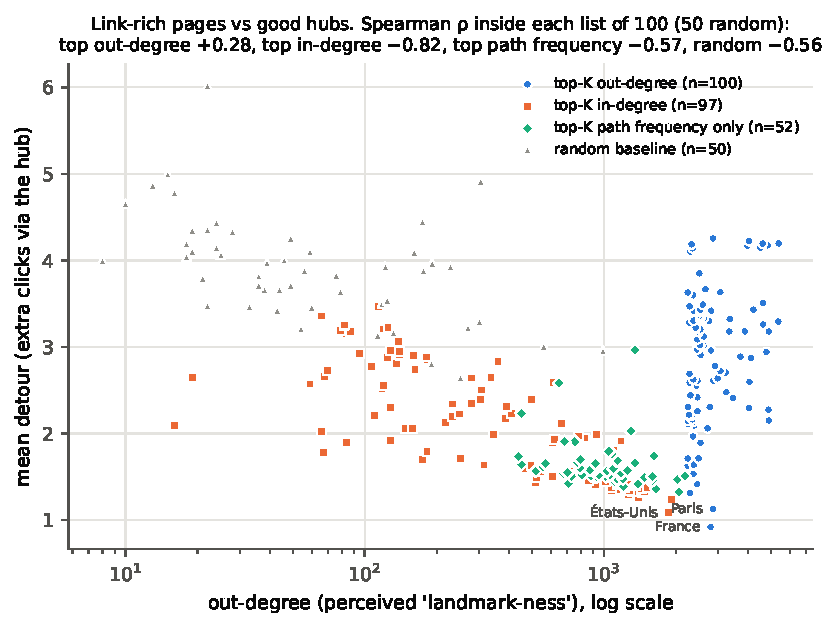
\includegraphics[width=\linewidth]{fig_detour_vs_outdegree.pdf}\caption{Out-degree vs mean detour.}\end{subfigure}\hfill
\begin{subfigure}{0.49\textwidth}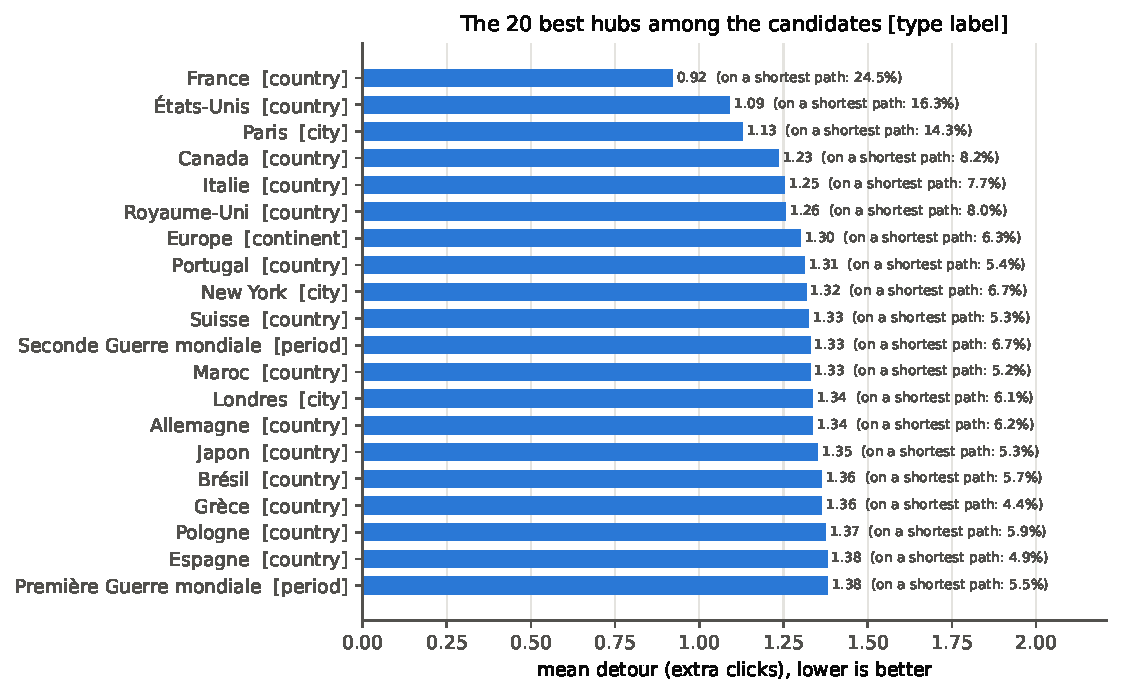
\includegraphics[width=\linewidth]{fig_best_hubs.pdf}\caption{Best 20 hubs.}\end{subfigure}\\[2pt]
\begin{subfigure}{0.49\textwidth}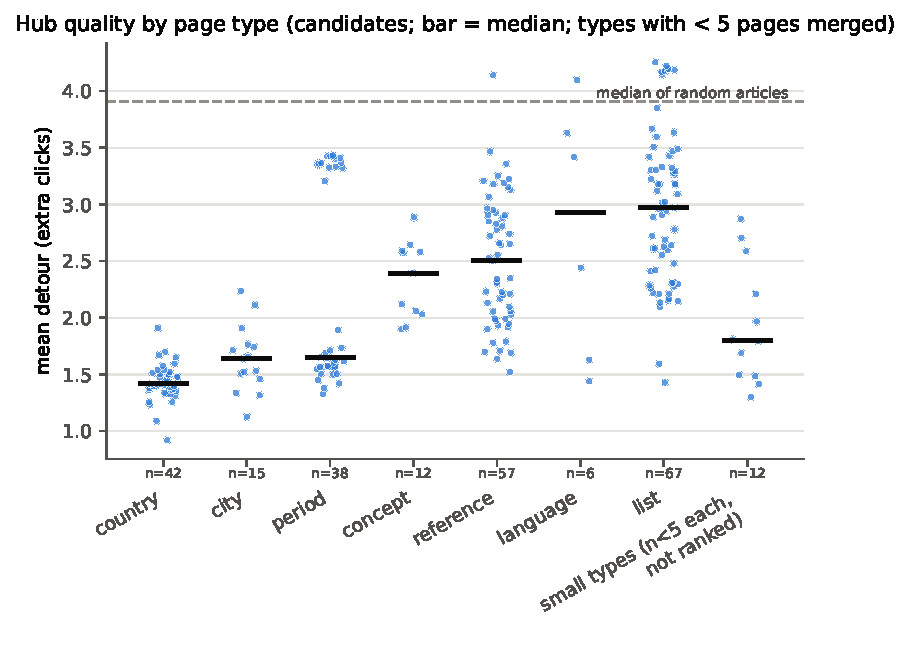
\includegraphics[width=\linewidth]{fig_detour_by_type.pdf}\caption{Hub quality by type label (non-random candidates).}\end{subfigure}\hfill
\begin{subfigure}{0.49\textwidth}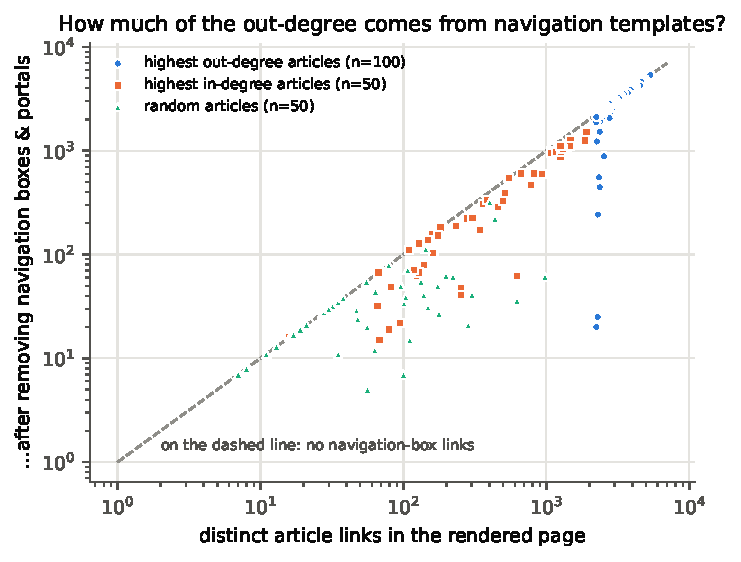
\includegraphics[width=\linewidth]{fig_bias_check.pdf}\caption{Template links in rendered pages.}\end{subfigure}
\caption{Perceived vs real hubs. Mean detour = extra clicks needed when the path must go through
the page, averaged over the \NReachable{} reachable random pairs.}
\label{fig:main}
\end{figure}

\begin{table}[t]\centering\small
\begin{tabular}{@{}rlp{1.5cm}rrrr@{}}
\toprule
\# & Page & Type & Out-deg. & In-deg. & Mean detour & On s.p. \\
\midrule
1 & France & country & 2{,}789 & 555{,}633 & 0.92 & 24.5\% \\
2 & États-Unis & country & 1{,}865 & 408{,}575 & 1.09 & 16.3\% \\
3 & Paris & city & 2{,}859 & 166{,}272 & 1.13 & 14.3\% \\
4 & Canada & country & 1{,}911 & 130{,}782 & 1.23 & 8.2\% \\
5 & Italie & country & 1{,}380 & 150{,}382 & 1.25 & 7.7\% \\
6 & Royaume-Uni & country & 1{,}397 & 164{,}371 & 1.26 & 8.0\% \\
7 & Europe & continent & 1{,}267 & 86{,}721 & 1.30 & 6.3\% \\
8 & Portugal & country & 2{,}282 & 38{,}238 & 1.31 & 5.4\% \\
9 & New York & city & 1{,}449 & 66{,}687 & 1.32 & 6.7\% \\
10 & Suisse & country & 1{,}314 & 82{,}905 & 1.33 & 5.3\% \\
11 & Seconde Guerre mondiale & period & 1{,}477 & 97{,}411 & 1.33 & 6.7\% \\
12 & Maroc & country & 2{,}055 & 29{,}004 & 1.33 & 5.2\% \\
13 & Londres & city & 1{,}280 & 75{,}069 & 1.34 & 6.1\% \\
14 & Allemagne & country & 1{,}076 & 158{,}591 & 1.34 & 6.2\% \\
15 & Japon & country & 1{,}167 & 93{,}395 & 1.35 & 5.3\% \\
\bottomrule
\end{tabular}

\caption{The 15 best candidate hubs (lowest mean detour). ``On s.p.'' = share of pairs for which the page lies on at least one shortest path.}
\label{tab:best}
\end{table}

\subsection{Interpretation}
\begin{itemize}
\item \textbf{The answer depends on what "landmark" means.}
  \begin{itemize}
  \item If landmarks are the \emph{kinds} of pages players aim for (countries, capitals,
    continents, world wars), intuition is largely right: these are the best hubs we found, with
    \BestHub{} far ahead.
  \item If landmarks are "pages with many links", intuition is wrong. Out-degree mostly measures
    \emph{list-ness}, and a long list of cantons leads everywhere \emph{in its niche} but is far
    from the rest of the encyclopedia.
  \end{itemize}
\item \textbf{What makes a good hub is being linked \emph{from} everywhere.} A page that many
  articles link to is close to almost every start. A broad page also links to sub-topics that are
  close to many targets. Countries combine both properties, while lists have only the second, and
  only locally.
\item \textbf{Template links are a double-edged signal.} They are a large share of ordinary pages'
  links. \emph{Reference} pages are probably reached mostly through templates and infoboxes (not
  measured), which makes them look central by in-degree. Those
  pages are nonetheless mediocre hubs: in-degree is a better proxy than out-degree, but not a
  perfect one.
\item These interpretations concern the structural \emph{optimum}. They do not describe how humans
  actually play: we used no game logs.
\end{itemize}

\section{Limitations}
\begin{itemize}
\item \textbf{Sampling.} An independent sample of \NPairs{} pairs (seed \OtherSeed) gives the same
  15 best hubs \SeedTopFifteenOrder{} and a rank correlation of \SeedRho{} on the \SeedN{} candidates
  evaluated in both, so sampling noise is small at this size. The
  path-frequency criterion relies on one sampled shortest path per pair, which is not uniform over
  all shortest paths. The \TopK-th candidate appears \PathFreqKth{} times among
  \NDistinctOnPaths{} distinct intermediate pages. This criterion is only used to \emph{find}
  candidates.
\item \textbf{Candidate set.} Hubs are evaluated only among \NCandidates{} candidates, so a better
  hub outside this set cannot be excluded.
\item \textbf{Labels.} The type labels are a judgement on page titles (assigned by hand, re-read
  once), and some categories are small.
\item \textbf{Model of the game.}
  \begin{itemize}
  \item The graph is unweighted and directed. It ignores where a link sits on the page, which
    matters for humans.
  \item Template links are kept as legal moves.
  \item The bias check renders old revisions with current templates.
  \end{itemize}
\item \textbf{Scope.} The statistics are descriptive. $p$-values are reported for information
  only, and we make no causal claim.
\end{itemize}

\section{Lessons learned}
\begin{itemize}
\item Never assume a schema. The 2026 dumps silently changed their layout, which a strict parser
  caught immediately.
\item Measure before cleaning. Redirect chains turned out to be trivial (maximum length 3), while
  red links and other namespaces mattered far more.
\item A systematic code review before the final run found 11 real defects: cache invalidation,
  mixed denominators, a unit mismatch in the bias check, and others. All were fixed before the
  final numbers.
\item Simple tools fitted the scale: \NArticles{} nodes in \CsrDiskGB\,GB of NumPy arrays. A graph database
  would have added a server without speeding up our queries.
\end{itemize}
\end{document}
